\documentclass[11pt]{exam}
\usepackage{listings}
\usepackage{pdfsync}

%
%  Created by Brad Miller on 2005-05-13.
%  Copyright (c) 2005 Luther College. All rights reserved.
%
%

\newif\ifpdf
\ifx\pdfoutput\undefined
\pdffalse % we are not running PDFLaTeX
\else
\pdfoutput=1 % we are running PDFLaTeX
\pdftrue
\fi

\ifpdf
\usepackage{subfigure}
\usepackage[pdftex]{graphicx}
\else
\usepackage{graphicx}
\fi

%
%  Update these values for running headers
%
\firstpageheader{\bf\Large CS-151}{\bf\Large Final Exam}{\bf\Large
  May 15, 2007 }
\runningheader{CS 151}{}{Final Exam}
\addpoints

\begin{document}

\begin{center} 
  \fbox{\fbox{\parbox{5.5in}{\centering This Exam is being given under
        the guidelines of the \textbf{Honor Code}. You are expected to
        respect those guidelines and to report those who do not.
        Answer the questions in the spaces provided. If you run out of
        room for an answer, continue on the back of the page.  There are
      \numquestions\  questions for a total of  \numpoints\ points.}}}
\end{center} 

% setup standard options for the including code fragments
\lstset{language=Python,numbers=left}

\vspace{0.1in} 
\hbox to \textwidth{Name:\enspace\hrulefill} 

% Questions start here:
\begin{questions}

\question Given the following list of numbers \lstinline{x = [13, 24, 5, 7, 9, 17, 32, 27, 2]}

\begin{parts}
\part[10]  Create a binary search tree and insert each of the numbers.  Show the final tree.
\vspace{3in}
\part[10]  Create a binary min-heap and insert the numbers one at a time into the heap. Show both the tree and list representation of the heap after all the numbers are inserted.
\vspace{3in}
\end{parts}

\newpage
\question Given the binary tree shown below:
\begin{figure}[h!]
    \begin{center}
        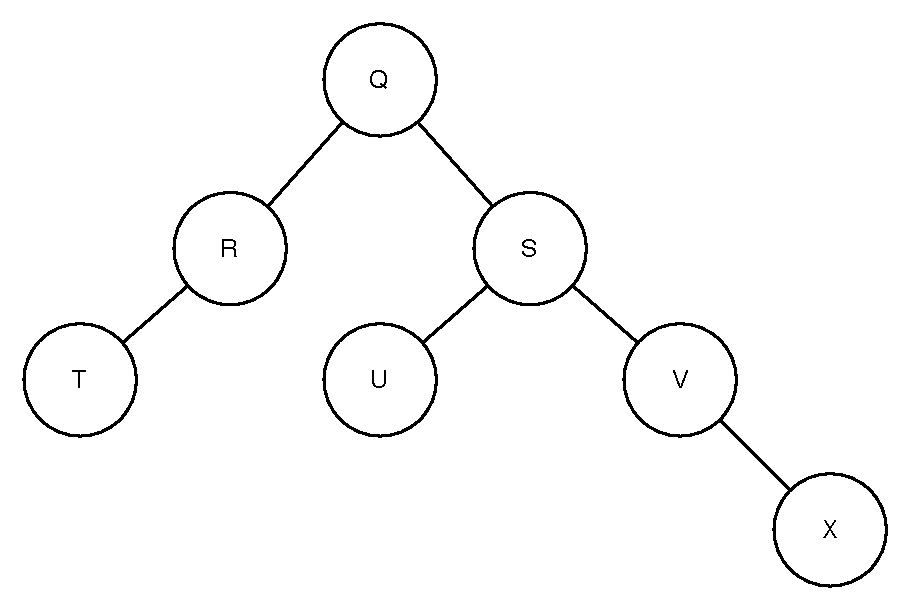
\includegraphics[height=3in]{binaryTree}
    \end{center}
\end{figure}
\begin{parts}
    \part[5] Perform a pre-order traversal of the tree.  Write out the name of each node in the order it is visited.
    \vspace{1in}
    \part[5] Perform a post-order traversal of the tree. Write out the name of each node in the order it is visited. 
    \vspace{1in}
\end{parts}

\newpage
\question
Yertlenet is a primitive form of networking that was used at Luther college up until the mid 1980's.  Yertlenet uses turtles as a message transport mechanism and requires that special one-way channels be dug between the buildings on campus to facilitate turtle navigation. A Messages is routed from building $x$ to building $y$ by placing a message on the back of a turtle and setting the turtle in the channel leading to the next building.  To facilitate routing, each building employed a student worker to receive incoming messages and if necessary move the turtle to the channel leading to the next building.  

You have just been hired as the new student worker for building one. Being a CS major you decide that you want to be the best turtle router on campus and therefore will create a graph of Yertlenet and figure out the optimum routing for messages that come through your building. The following table shows the information describing the Yertlenet connections. Column one is the start building, column two is the end building, and column three is the cost of the link.

\begin{verbatim}
1 2 10
1 3 15
1 6 5
2 3 2
3 4 7
3 6 10
4 5 7
6 4 5
5 6 13
\end{verbatim}

\begin{parts}
\part[5]
Draw the directed graph represented by the above table.

\part[10]
Using Dijkstras algorithm, find the shortest path from each other building on campus to yours.  Make sure that you show the contents of the priority queue you run the algorithm, and fill in the predecessor links on the graph using dashed lines.
\vspace{6in}
\end{parts}

\newpage
\question[10]  Recall that the height of the tree is defined as the number of edges between the root and the deepest leaf in the tree.  Write a function height(t) that takes a tree as a parameter and returns the height of the tree.  \textit{Hint 1:} The methods for a tree are as follows:
\begin{itemize}

	\item BinaryTree()  Create a new instance of a binary tree.
    \item getLeftChild() Return the binary tree corresponding to the left child of the current node.
    \item getRightChild() Return the binary tree corresponding to the right child of the current node.
    \item setRootVal(x) Store the object in parameter x in the current node.
    \item getRootVal() Return the object stored in the current node.
    \item insertLeft(x) Create a new binary tree and install it as the left child of the current node.
    \item insertRight(x) Create a new binary tree and install it as the right child of the current node.

\end{itemize}

\textit{Hint 2:} The height function is very simple (and short) if you think recursively.

\newpage
\question  Consider the following classic problem:  A farmer along with his fox, goose and a sack of oats are out for a walk.  They come to a river that they must cross.  The problem is that the boat is only large enough to hold the farmer and one additional object.  The goose cannot be left alone with the grain or it will eat all the grain.  The fox cannot be left alone with the goose or it will eat the goose.  The goose, fox, and oats are incapable of rowing.  Find a series  of crossings that will get everyone safely to the other side of the river.

This problem can be solved using a graph search algorithm.  The key is to recognize that the nodes in the graph represent a ``configuration'' of the problem, with certain things on one side of the river and certain things on the other.  Edges between nodes represent legal movements of items from one side to the other.

\begin{parts}
    \part[10]  Draw a graph to show the solution to this problem.

    
    \part[5]  Which Graph algorithm would you use to find the smallest number of crossings? 
\end{parts}
\vspace{8in}

%\question[10] Draw the expression tree for the expression $(8 * 7) / (4 + 3 * 5) - (16 * 3 + 4)$  
%\newpage
\question[10] Given the graph below find the minimal weight spanning tree for the graph produced by using Prim's algorithm. Start with vertex \textbf{a} Make sure you show the contents of the priority queue after each vertex is explored.  When you are done draw the spanning tree for the graph.
\begin{figure}[h!t]
        \begin{center}
        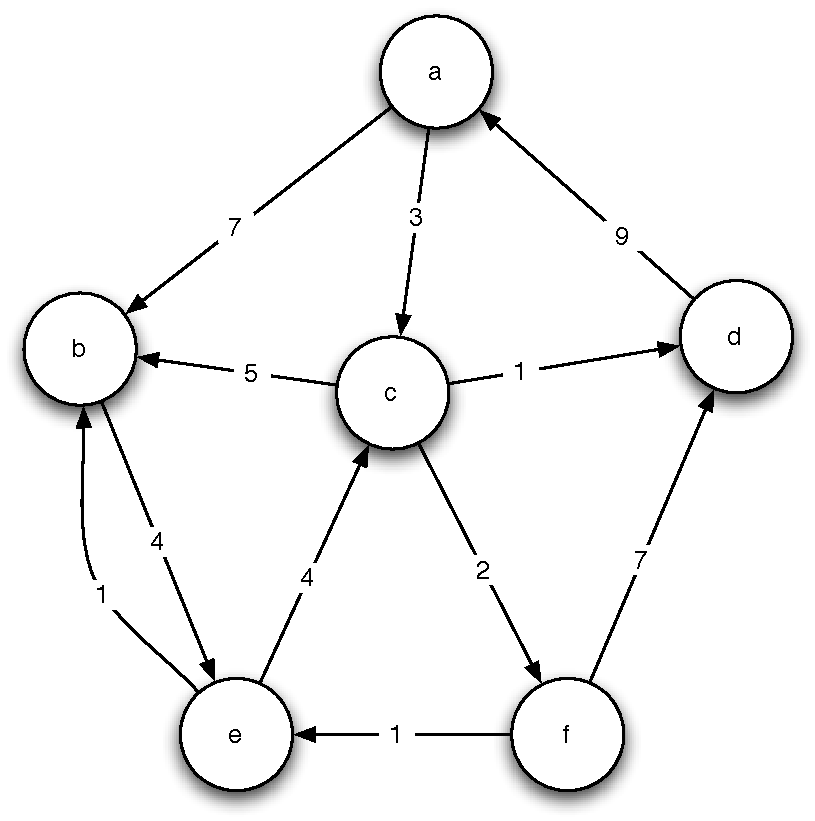
\includegraphics[scale=.75]{spanning}
    \end{center}
\end{figure}

\newpage
\question[10] Apply the depth first search algorithm to the graph below. Show the starting and finishing times for each vertex.  Draw in the  predecessor links for each vertex as well.  Start with node \textbf{a}.  You should assume that the vertices are stored in alphabetical order on the adjacency lists.
\begin{figure}[h!t]
        \begin{center}
        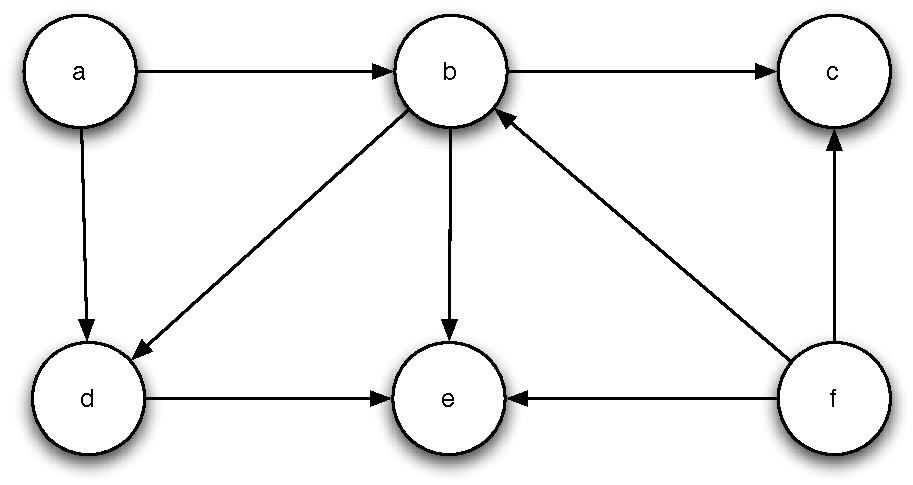
\includegraphics[scale=.75]{dfs}
    \end{center}
\end{figure}

\end{questions}

\end{document}

